\chapter{Evaluation}
\label{chap:evaluation}
in this chapter, we evaluate and compare various different settings

"We found crossover and mutation most influential in GA success."\cite{mills_determining_2015}

"The cross over operator is found to be the most influential parameter in both the case studies, followed by mutation rate, population size for case study-1 and population size and selection process for case study-2. It is evident that the robust GA parameter settings are sensitive"\cite{majumdar_genetic_2015}

\cite{boyabatli_parameter_2004} also suggest a high mutation rate.



It seams like the high variations does not allow for more complex traffic situations, giving a clear priority to pedestrian actions

TODO: chart: emergency break due to pedestrians vs vehicles


In the last chapter \ref{chap:hyperparameter_tuning}, values from the cost function (shown in section \ref{implementation:cost_function}) were displayed. These values however are difficult to interpret. Considering this, in this chapter, these values will be modified using this equation:

(3500 - cost) / 100

This will result in a value called Emergency Brake Duration, which will from now on be using instead of cost. The higher the Emergency Brake Duration, the better. It is important to consider, that this value might not exactly correspond to the actual Emergency Brake Duration time from the simulation, as the cost function applies a penalty for emergency breaks lasting longer then 3 seconds (again, see section \ref{implementation:cost_function}).






EFFECT SIZE:
From: Discovering Statistics using R
Effect sizes are useful because they provide an objective measure of the importance of an effect. So, it doesn’t matter what effect you’re looking for, what variables have been measured, or how those variables have been measured – we know that a correlation coefficient of 0 means there is no effect, and a value of 1 means that there is a perfect effect.
Cohen (1988, 1992) has also made some widely used suggestions about what constitutes a large or small effect: 
r = .10 (small effect): In this case the effect explains 1\% of the total variance. 
r = .30 (medium effect): The effect accounts for 9\% of the total variance. 
r = .50 (large effect): The effect accounts for 25\% of the variance.


From chat: 
Effect size, on the other hand, quantifies the strength or magnitude of an observed effect. It provides a standardized measure that allows researchers to assess the practical significance of their findings.
Effect size is not affected by sample size, making it a valuable metric for comparing the impact of different interventions or experimental conditions.

\section{Comparison with random and default ga Values}
scenario 1: default : 9v 5p
\begin{figure}[ht] 
	\label{figure:sim_1_comparison}
	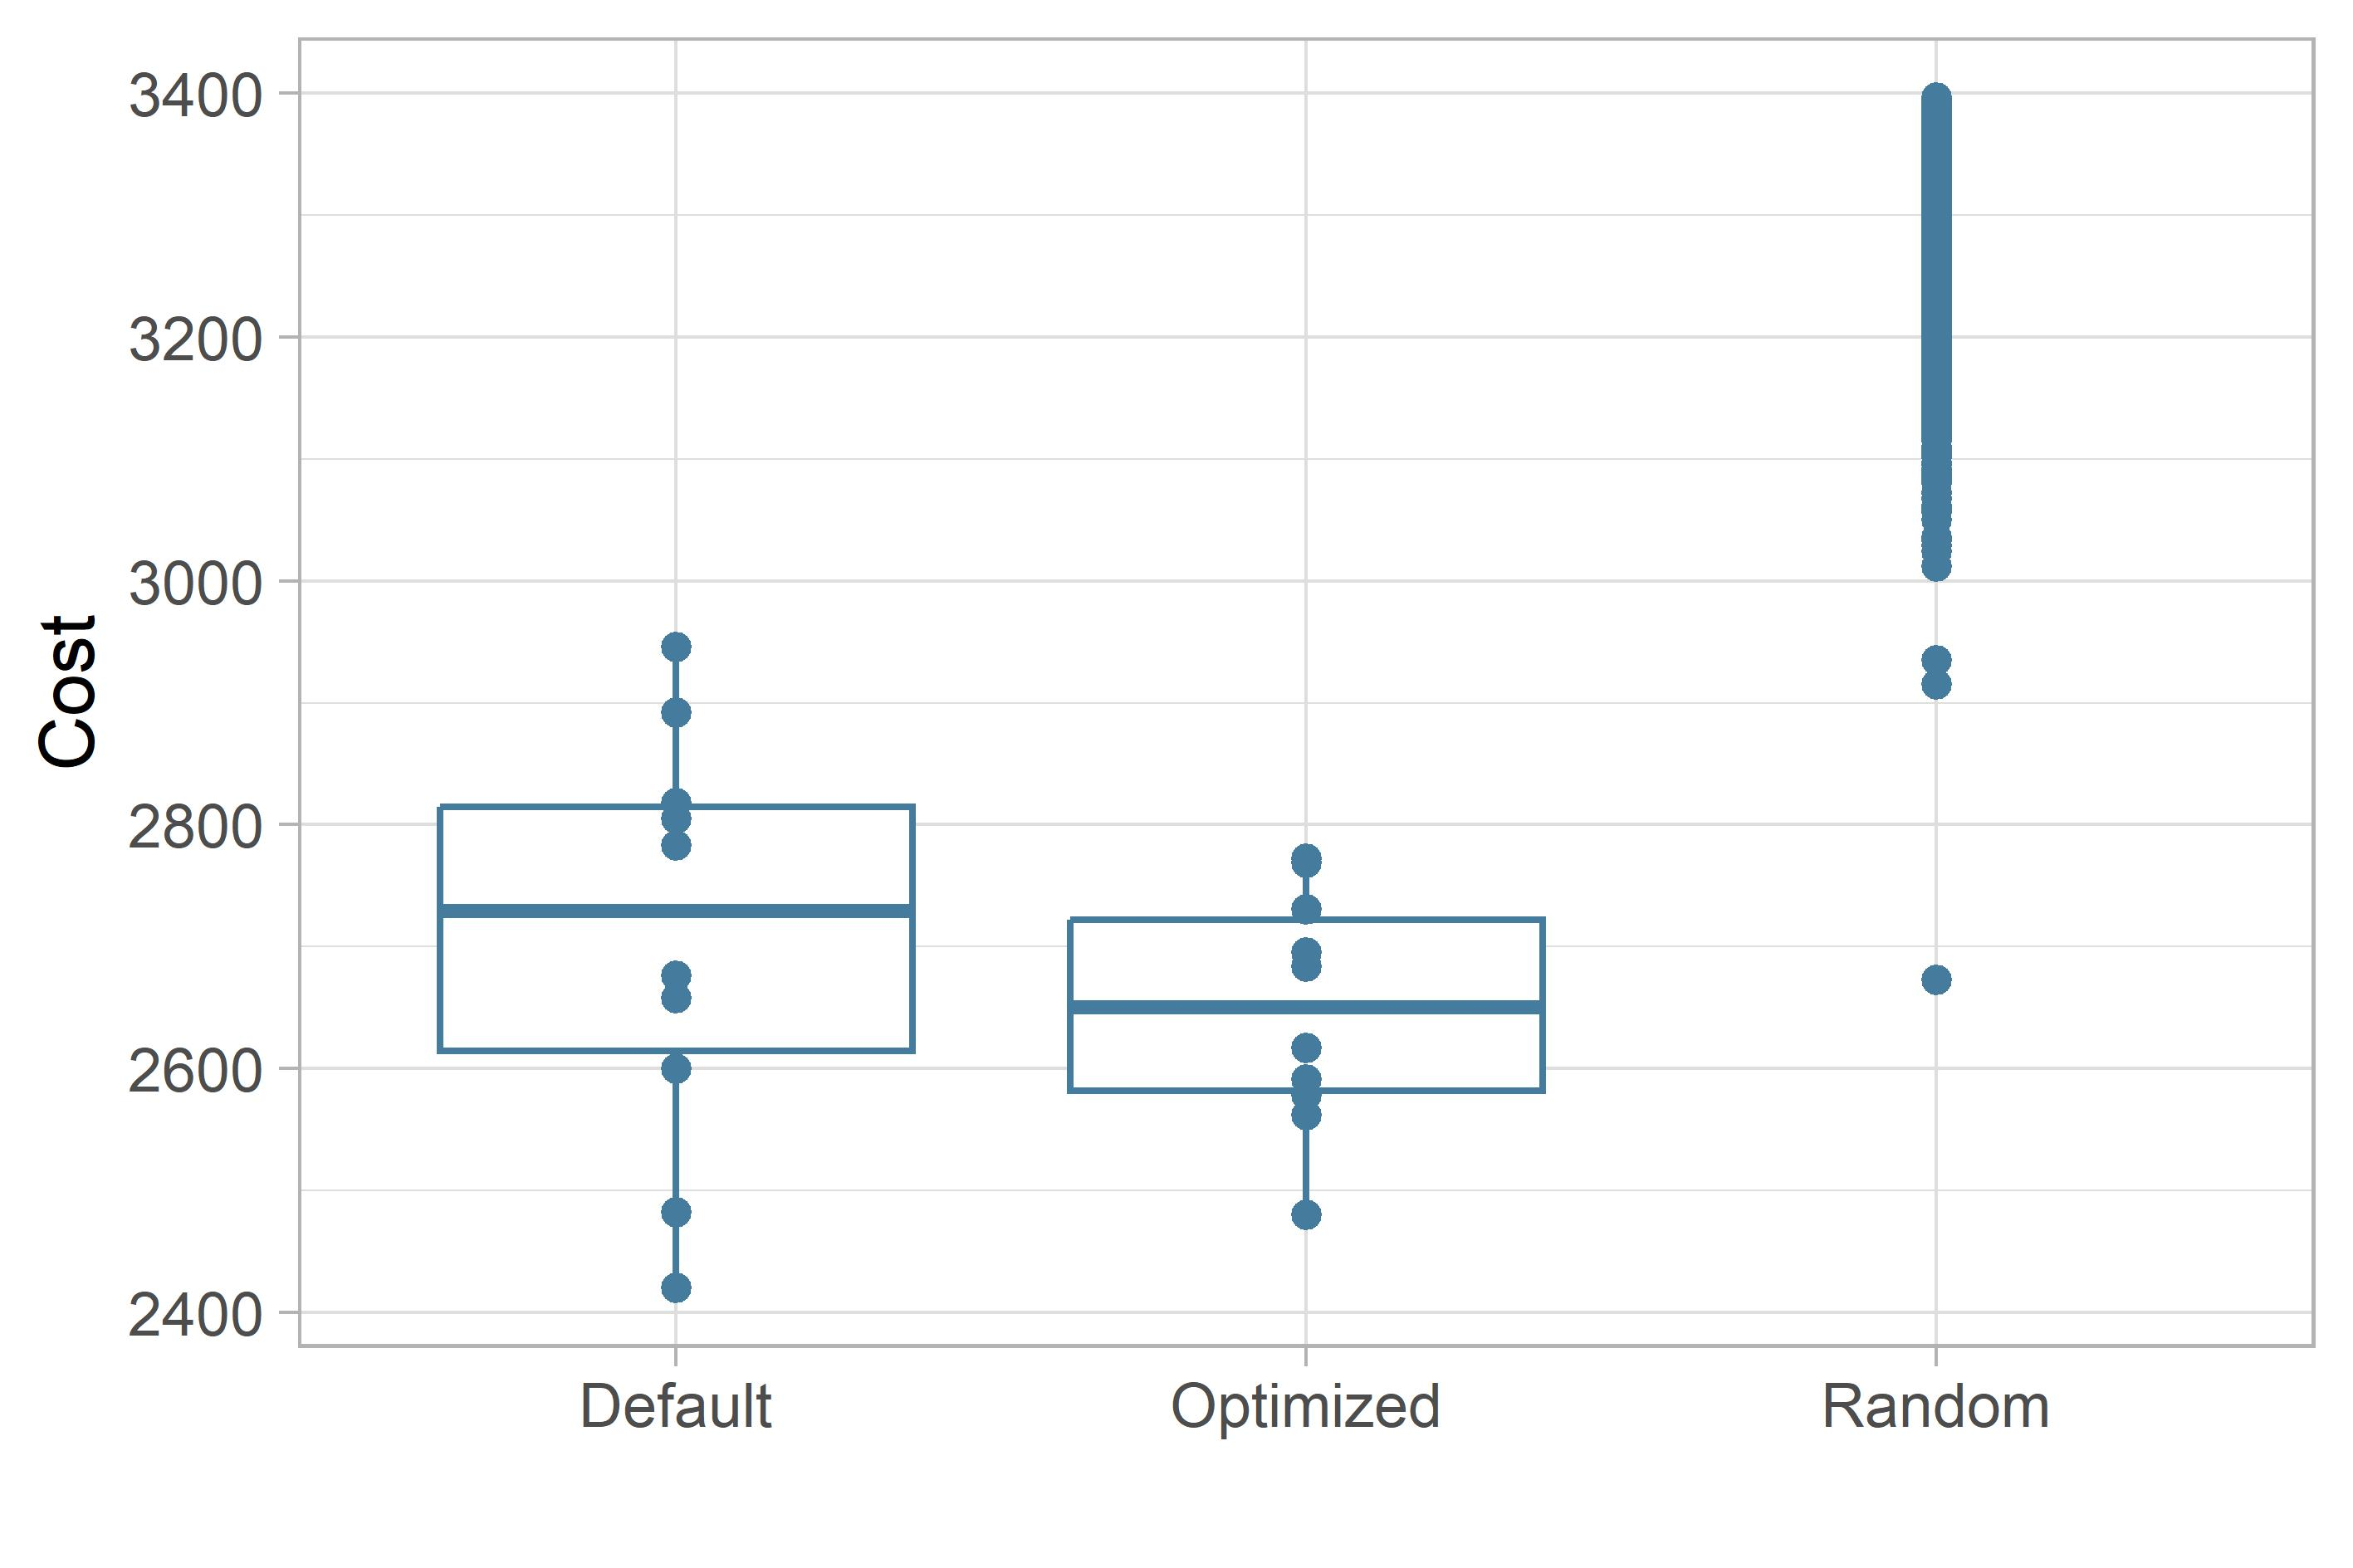
\includegraphics[width=1\linewidth]{simulations/evaluation/plots/sim_1_comparison}
	\caption{Comparison simulation 1: Default GA vs Optimized GA vs Random}
\end{figure}

\begin{figure}[ht] 
	\label{figure:sim_1_ga_comparison}
	\begin{minipage}[b]{0.5\linewidth}
		\centering
		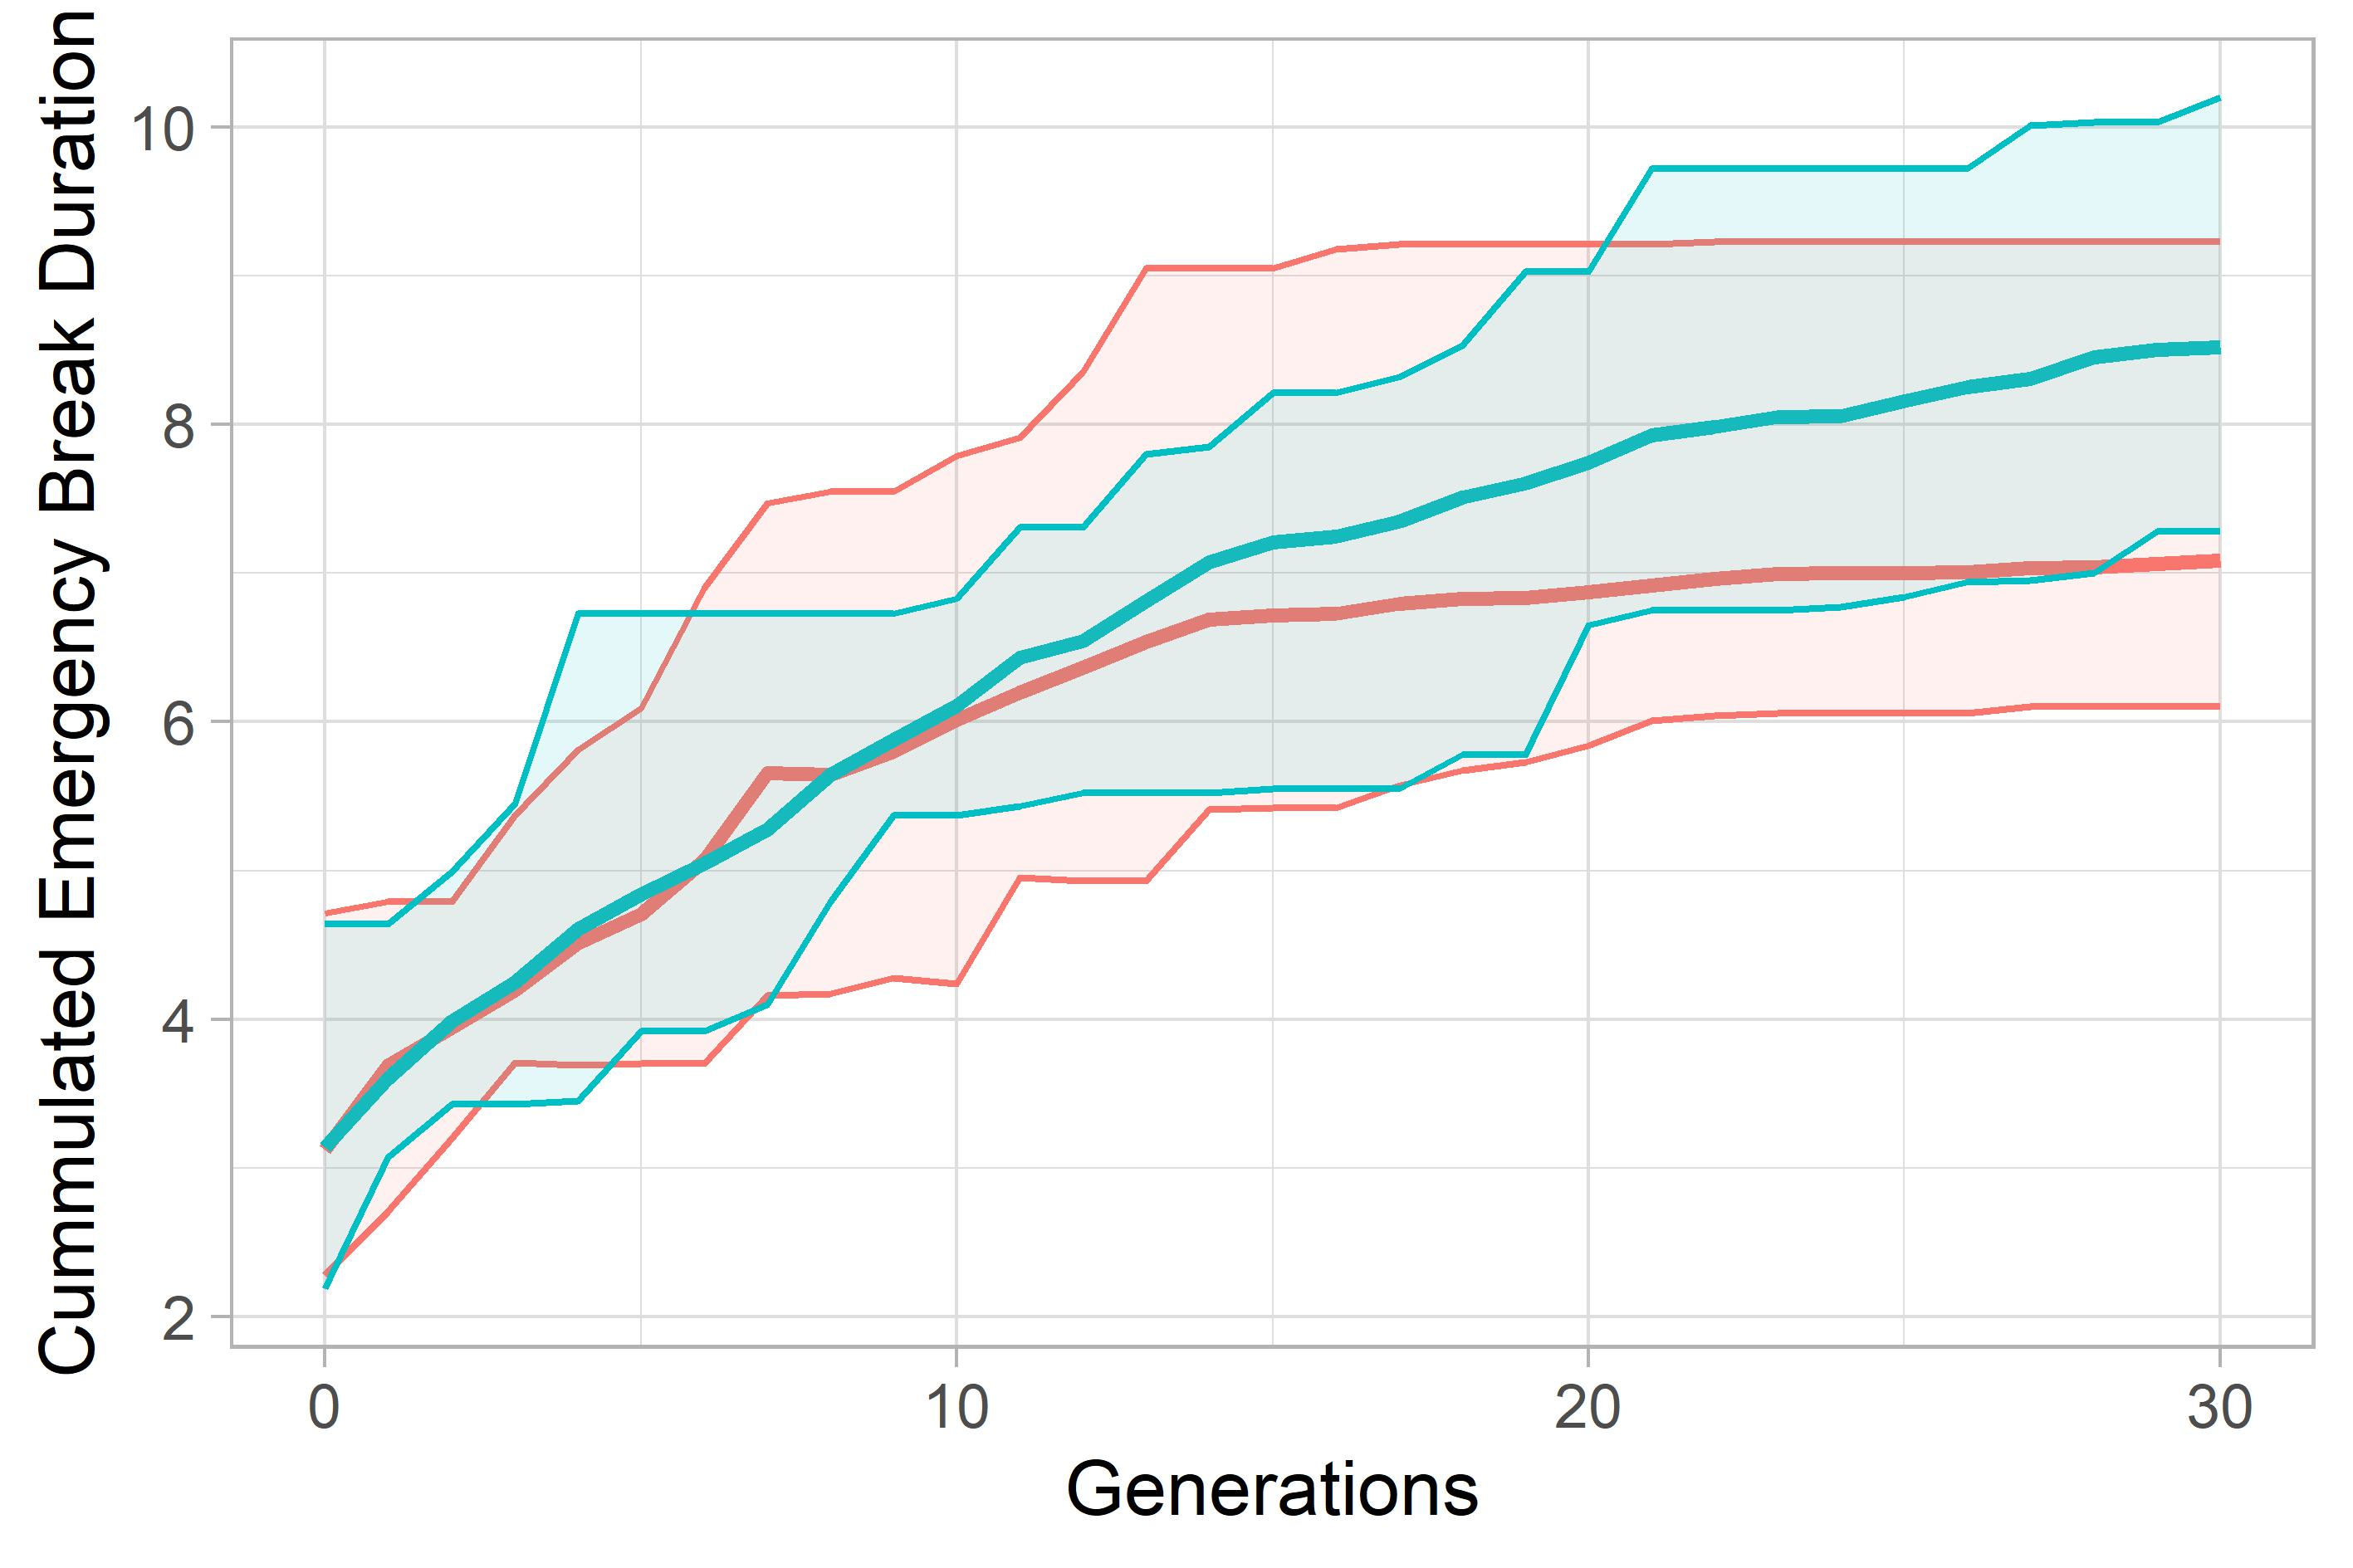
\includegraphics[width=1\linewidth]{simulations/evaluation/plots/sim_1_ga_generations} 
	\end{minipage}%%
	\begin{minipage}[b]{0.5\linewidth}
		\centering
		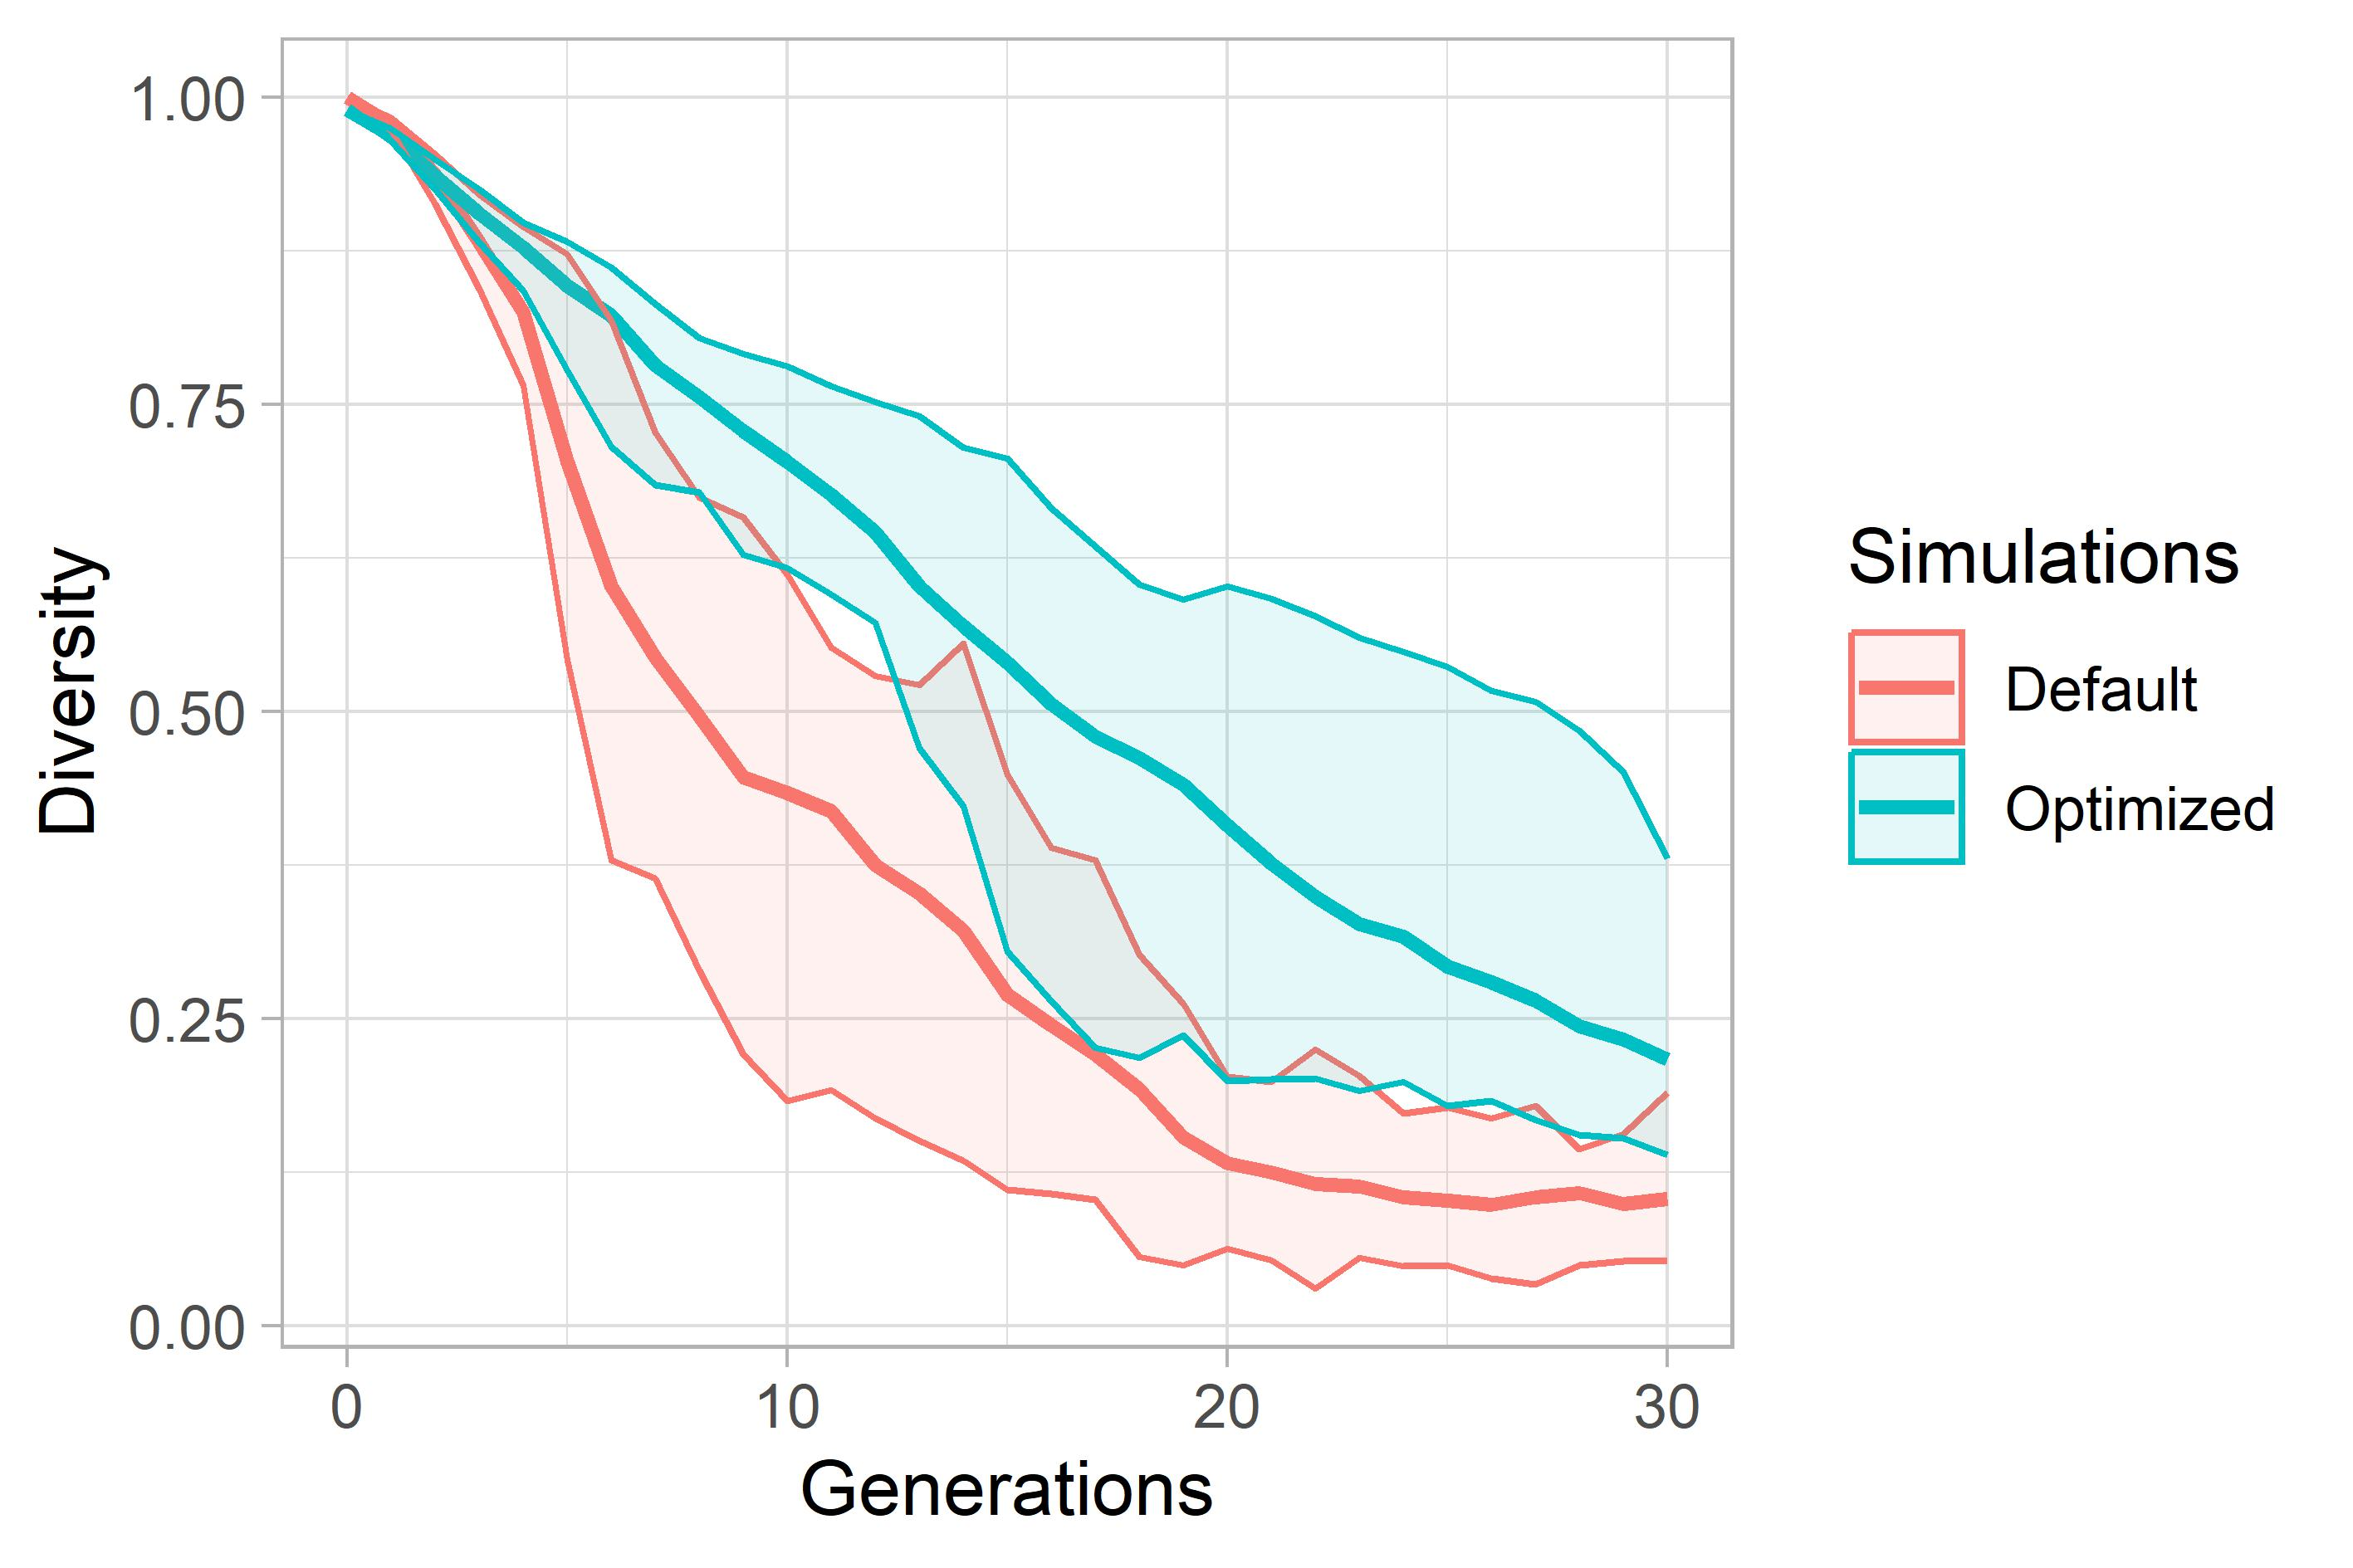
\includegraphics[width=1\linewidth]{simulations/evaluation/plots/sim_1_ga_diversity} 
	\end{minipage} 
	\caption{Comparison over generations. simulation 1}
\end{figure}


\section{Generalization on different start scenarios}

\subsubsection{Scenario 2}
scenario 2: 9v 5p
\begin{figure}[ht] 
	\label{figure:sim_2_comparison}
	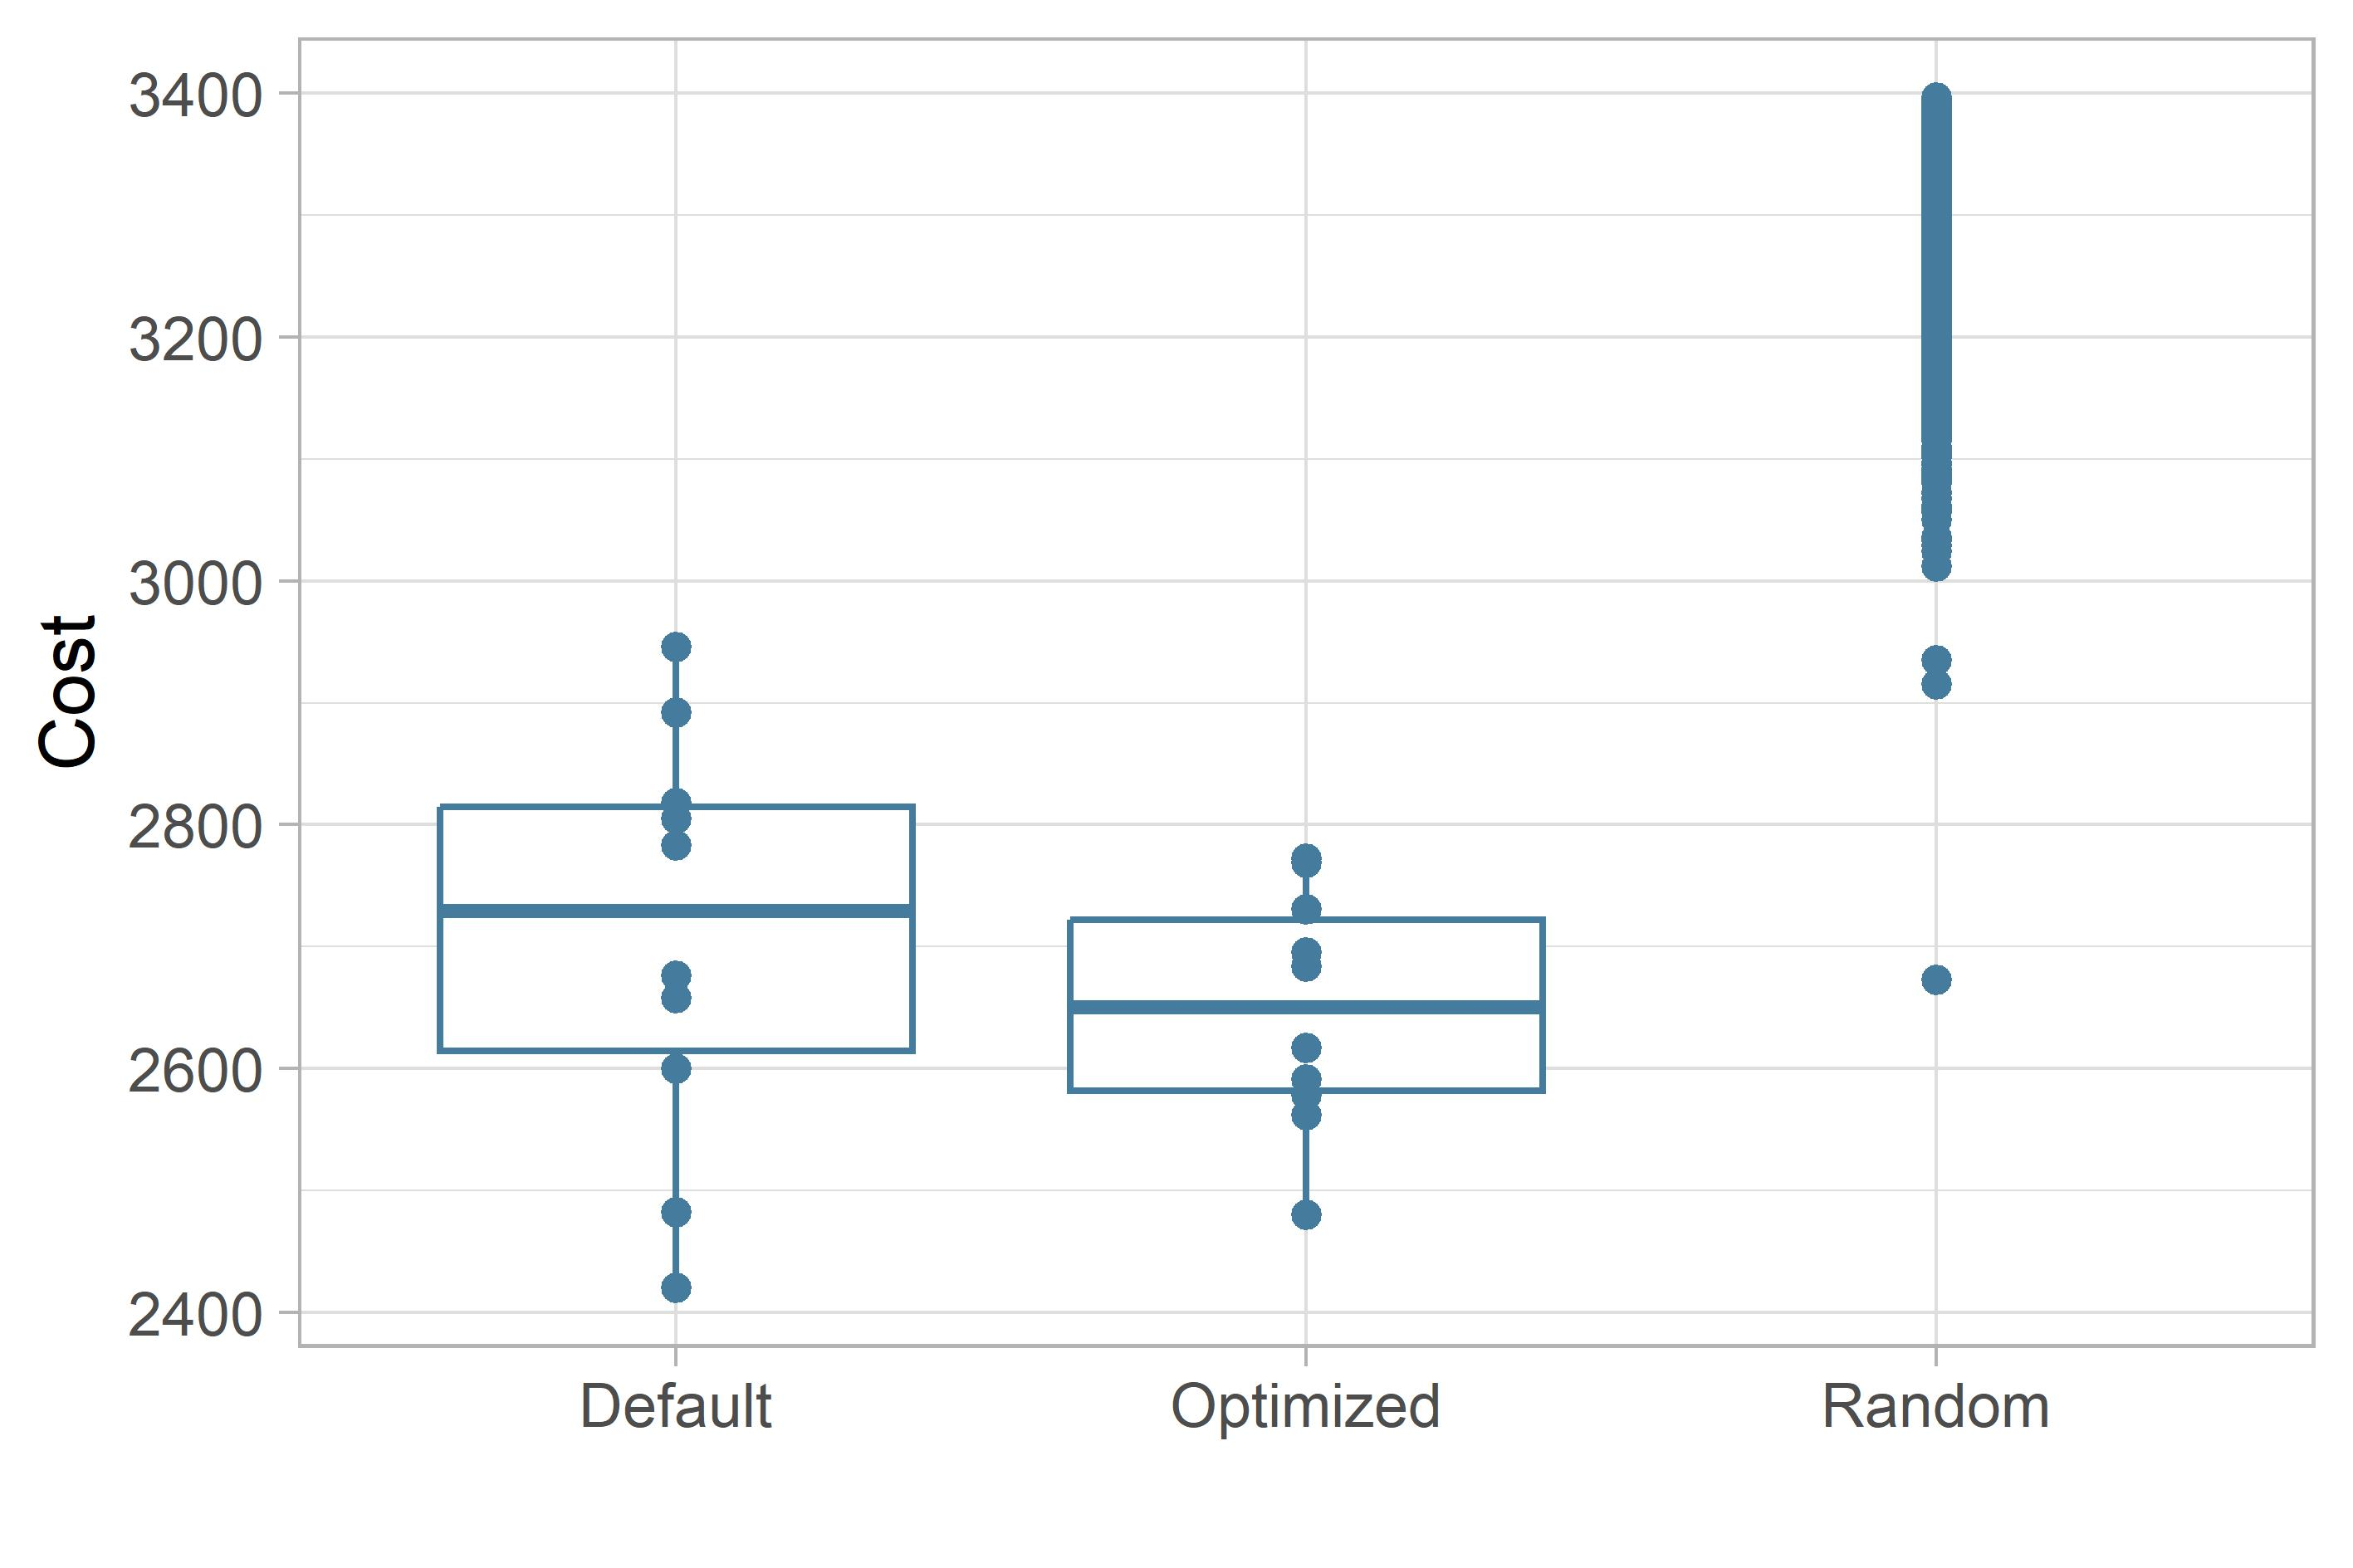
\includegraphics[width=1\linewidth]{simulations/evaluation/plots/sim_1_comparison}
	\caption{Genetic Algorithm with Elite}
\end{figure}


\subsubsection{Scenario 3}
scenario 3: 5v 3p
\begin{figure}[ht] 
	\label{figure:sim_3_comparison}
	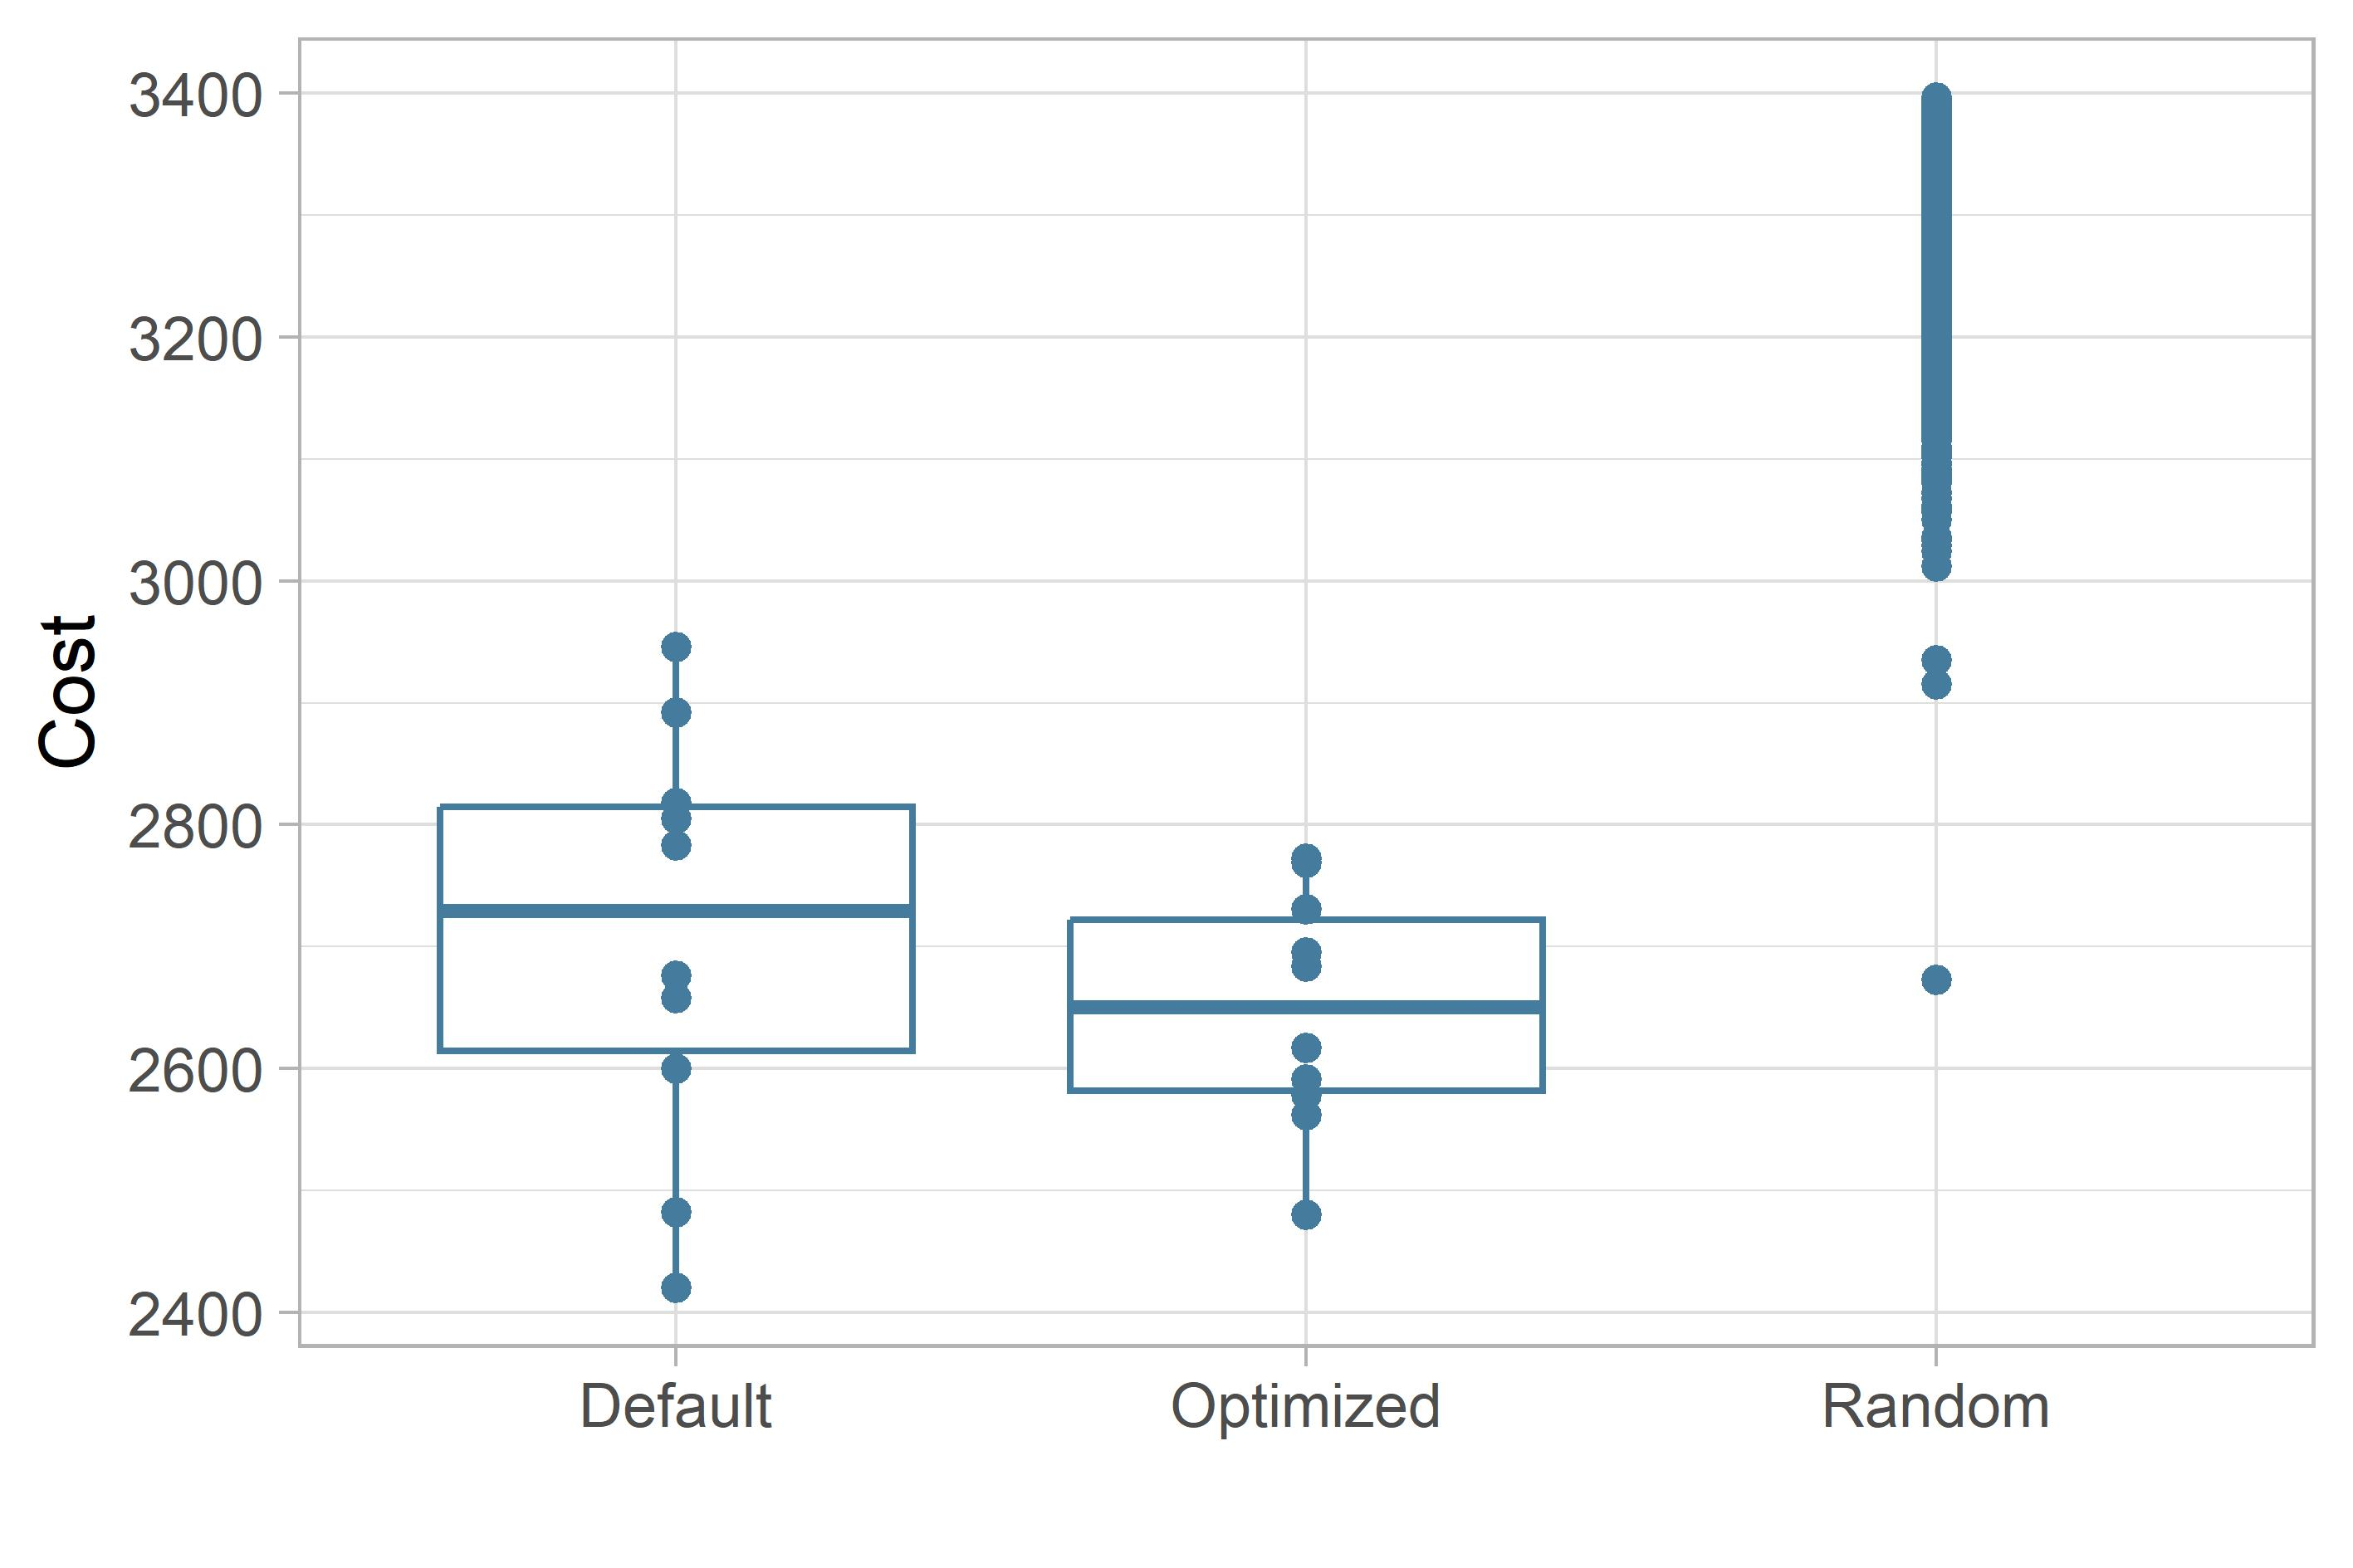
\includegraphics[width=1\linewidth]{simulations/evaluation/plots/sim_1_comparison}
	\caption{Genetic Algorithm with Elite}
\end{figure}

\subsubsection{Scenario 4}
scenario 4: 18v 10p
\begin{figure}[ht] 
	\label{figure:sim_4_comparison}
	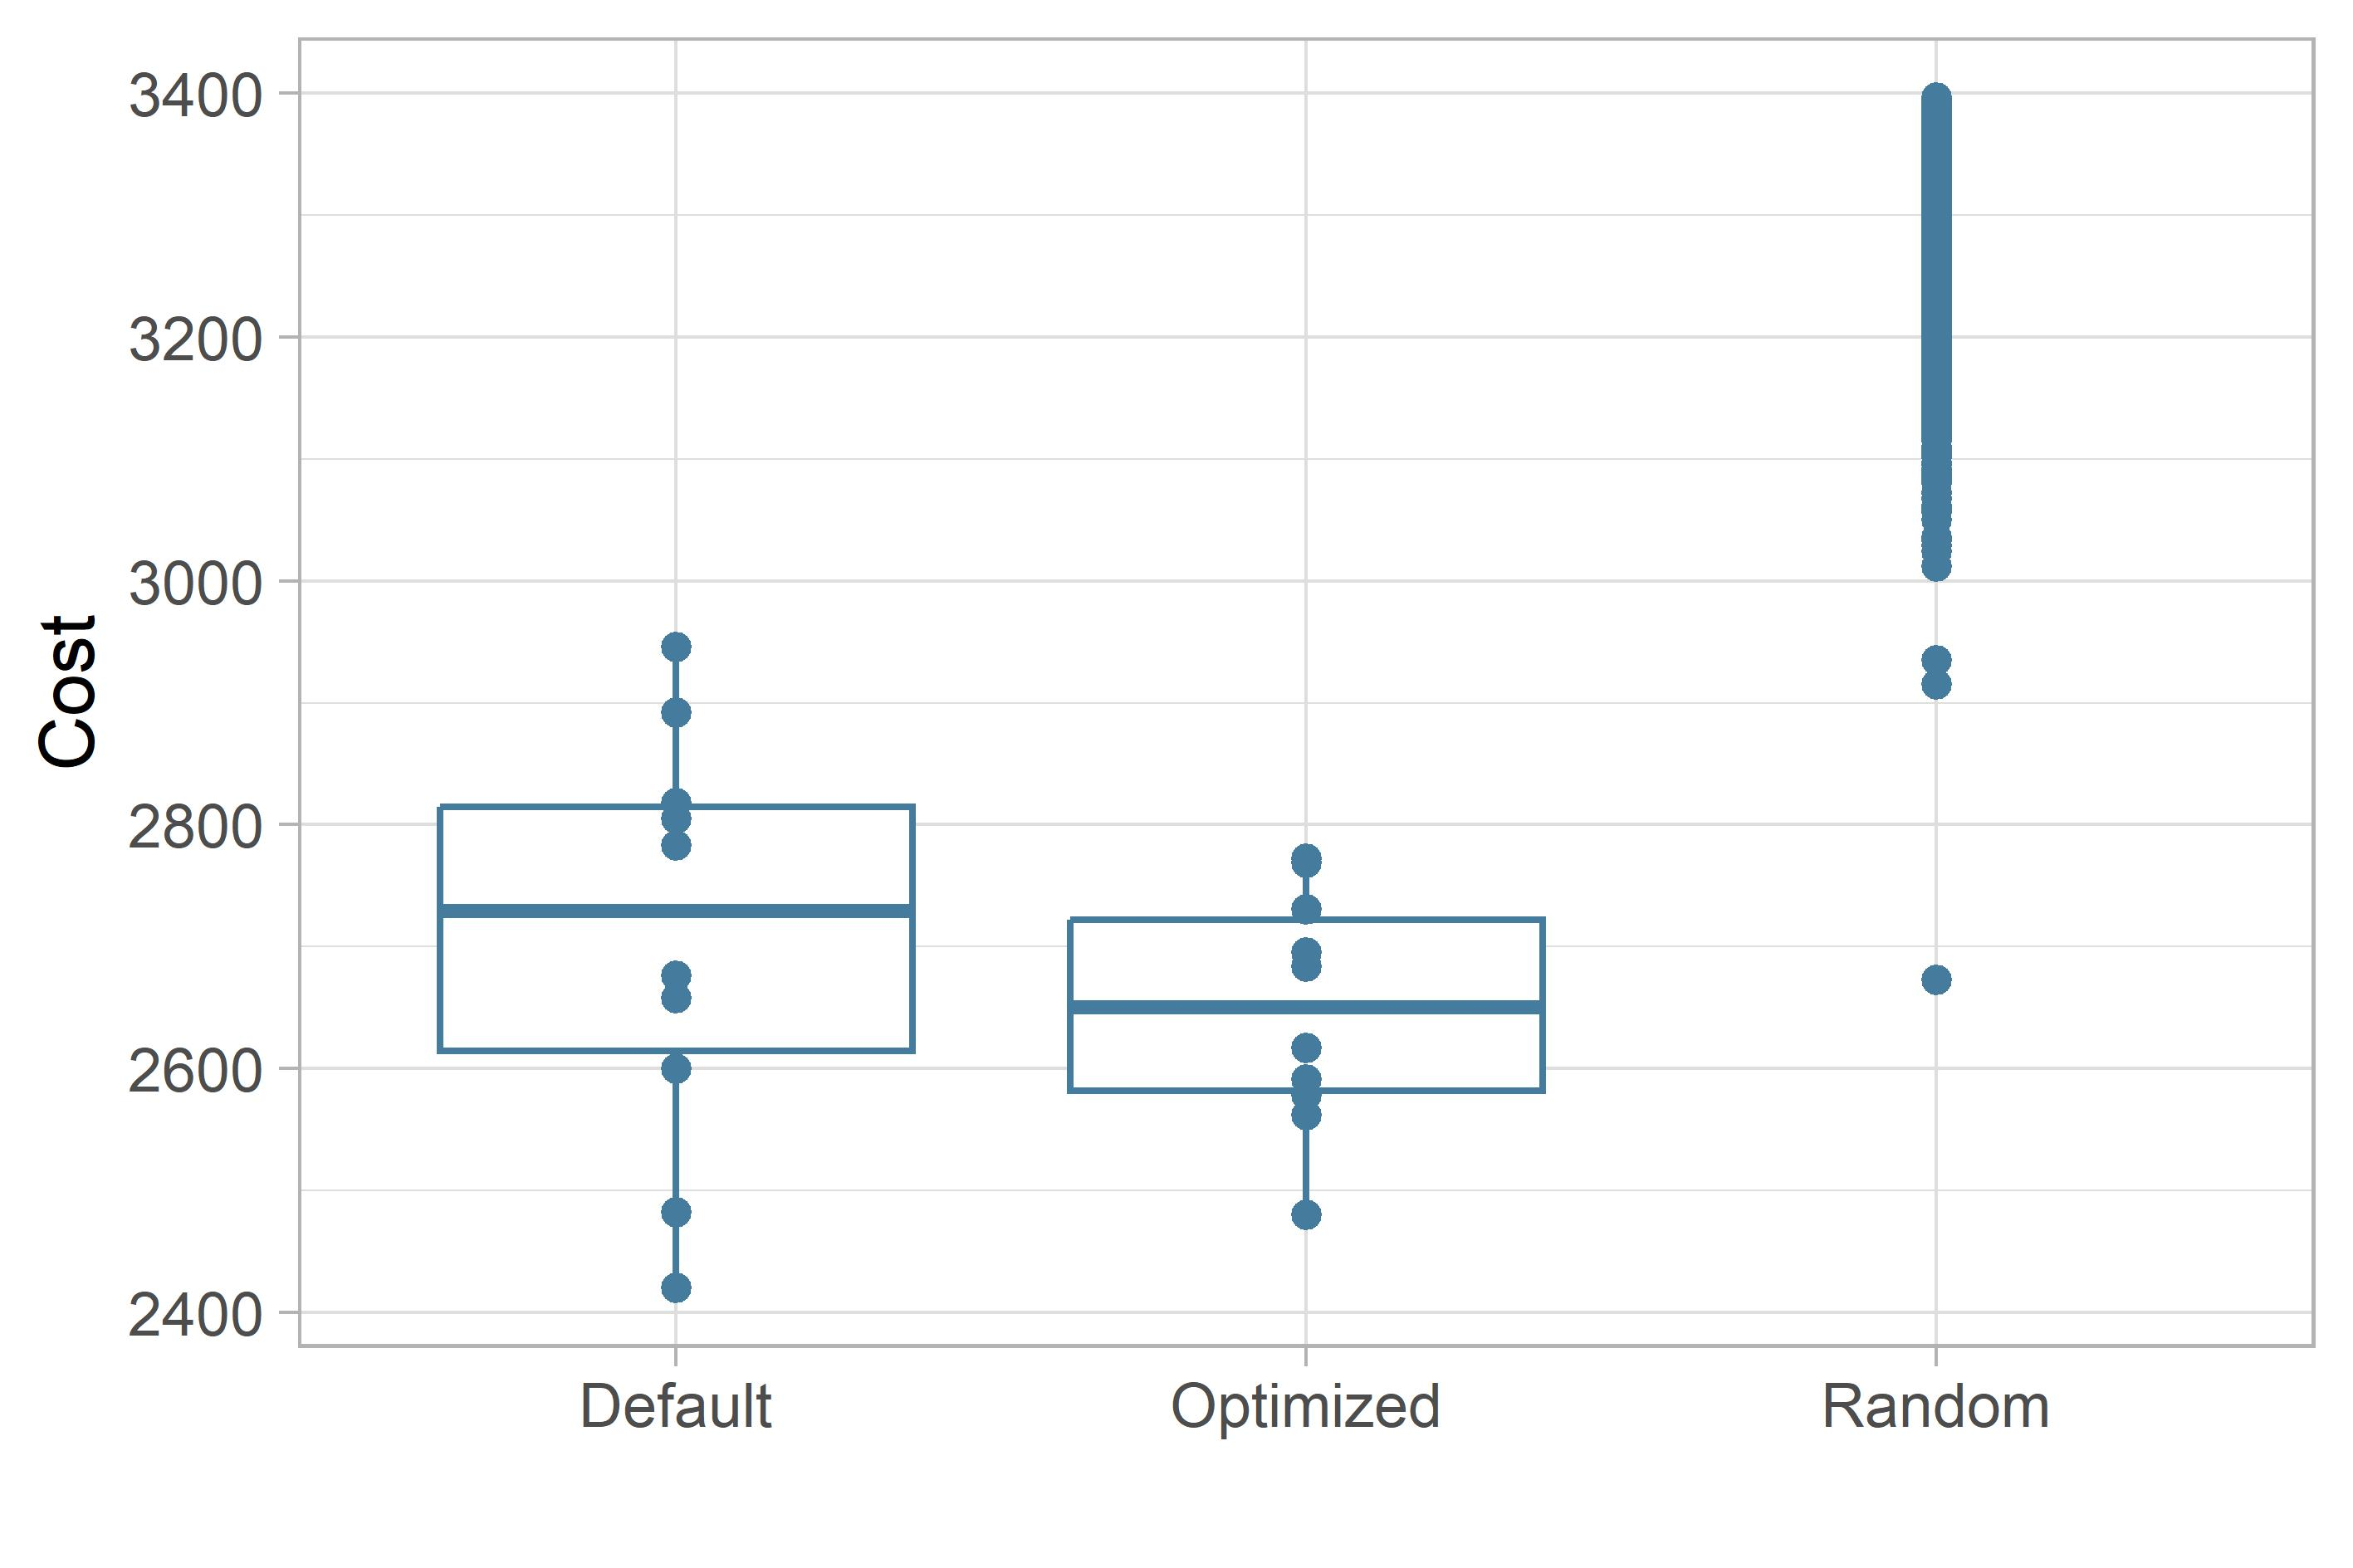
\includegraphics[width=1\linewidth]{simulations/evaluation/plots/sim_1_comparison}
	\caption{Genetic Algorithm with Elite}
\end{figure}



\todo{also compare (average) diversity?}